\subsubsection{Basis}
\begin{figure}[!htb]
    \centering
    \begin{subfigure}{.49\textwidth}
        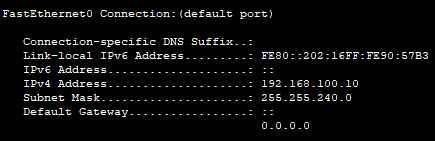
\includegraphics[width=\textwidth]{./img/build/pc0.png}
        \caption{PC0 - 192.168.100.10/20}
    \end{subfigure}
    \begin{subfigure}{.49\textwidth}
        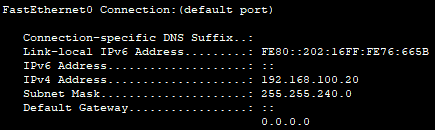
\includegraphics[width=\textwidth]{./img/build/pc1.png}
        \caption{PC1 - 192.168.100.20/20}
    \end{subfigure}
    ~
    \begin{subfigure}{.49\textwidth}
        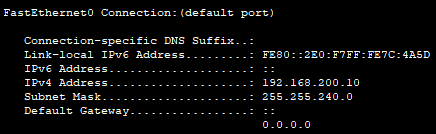
\includegraphics[width=\textwidth]{./img/build/pc2.png}
        \caption{PC2 - 192.168.200.10/20}
    \end{subfigure}
    \begin{subfigure}{.49\textwidth}
        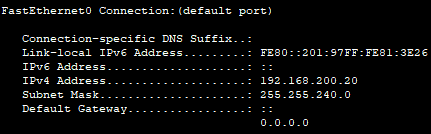
\includegraphics[width=\textwidth]{./img/build/pc3.png}
        \caption{PC3 - 192.168.200.20/20}
    \end{subfigure}
    \caption{Endsysteme}
\end{figure}

\subsubsection{Servernetzwerk}

\begin{figure}[!htb]
    \centering
    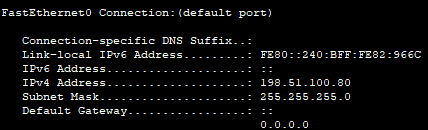
\includegraphics[width=\textwidth]{./img/build/server.png}
    \caption{Server}
\end{figure}

\pagebreak
\paragraph{index.html}
\begin{lstlisting}[language=HTML]
<!DOCTYPE html>
<html lang="en">
<head>
    <meta charset="utf-8" />
    <!--<link rel="icon" href="/favicon.ico" />-->
    <meta name="viewport" 
    content="width=device-width, initial-scale=1" />
    <script type="module">
    async () => {
    if(typeof IntersectionObserver === undefined){
        //import polyfill
        const intersectionPolyfill = 
        'https://cdn.jsdelivr.net/npm/
        intersection-observer@0.12.0/
        intersection-observer.min.js';
        
        window.IntersectionObserver = 
        (await import(intersectionPolyfill)).default;
        }
    };
    </script>
</head>
<body>
    <div id="svelte"></div>

    <script>
    const mount = document.getElementById("svelte");
    const h2 = document.createElement("h2");
    h2.innerText = "Shehata loves JS";
    mount.appendChild(h2);
    </script>
</body>
</html>
\end{lstlisting}

\begin{figure}[!htb]
    \centering
    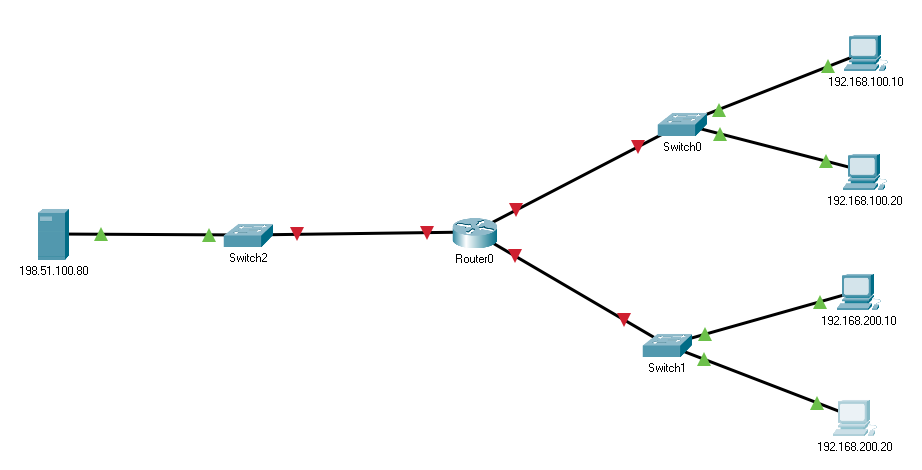
\includegraphics[width=\textwidth]{./img/build/start.png}
    \caption{Netzwerk}
\end{figure}